% Figure definitions for TempAnom-GNN paper

% Figure 1: Three-panel evaluation overview
\begin{figure*}[htbp]
\centering
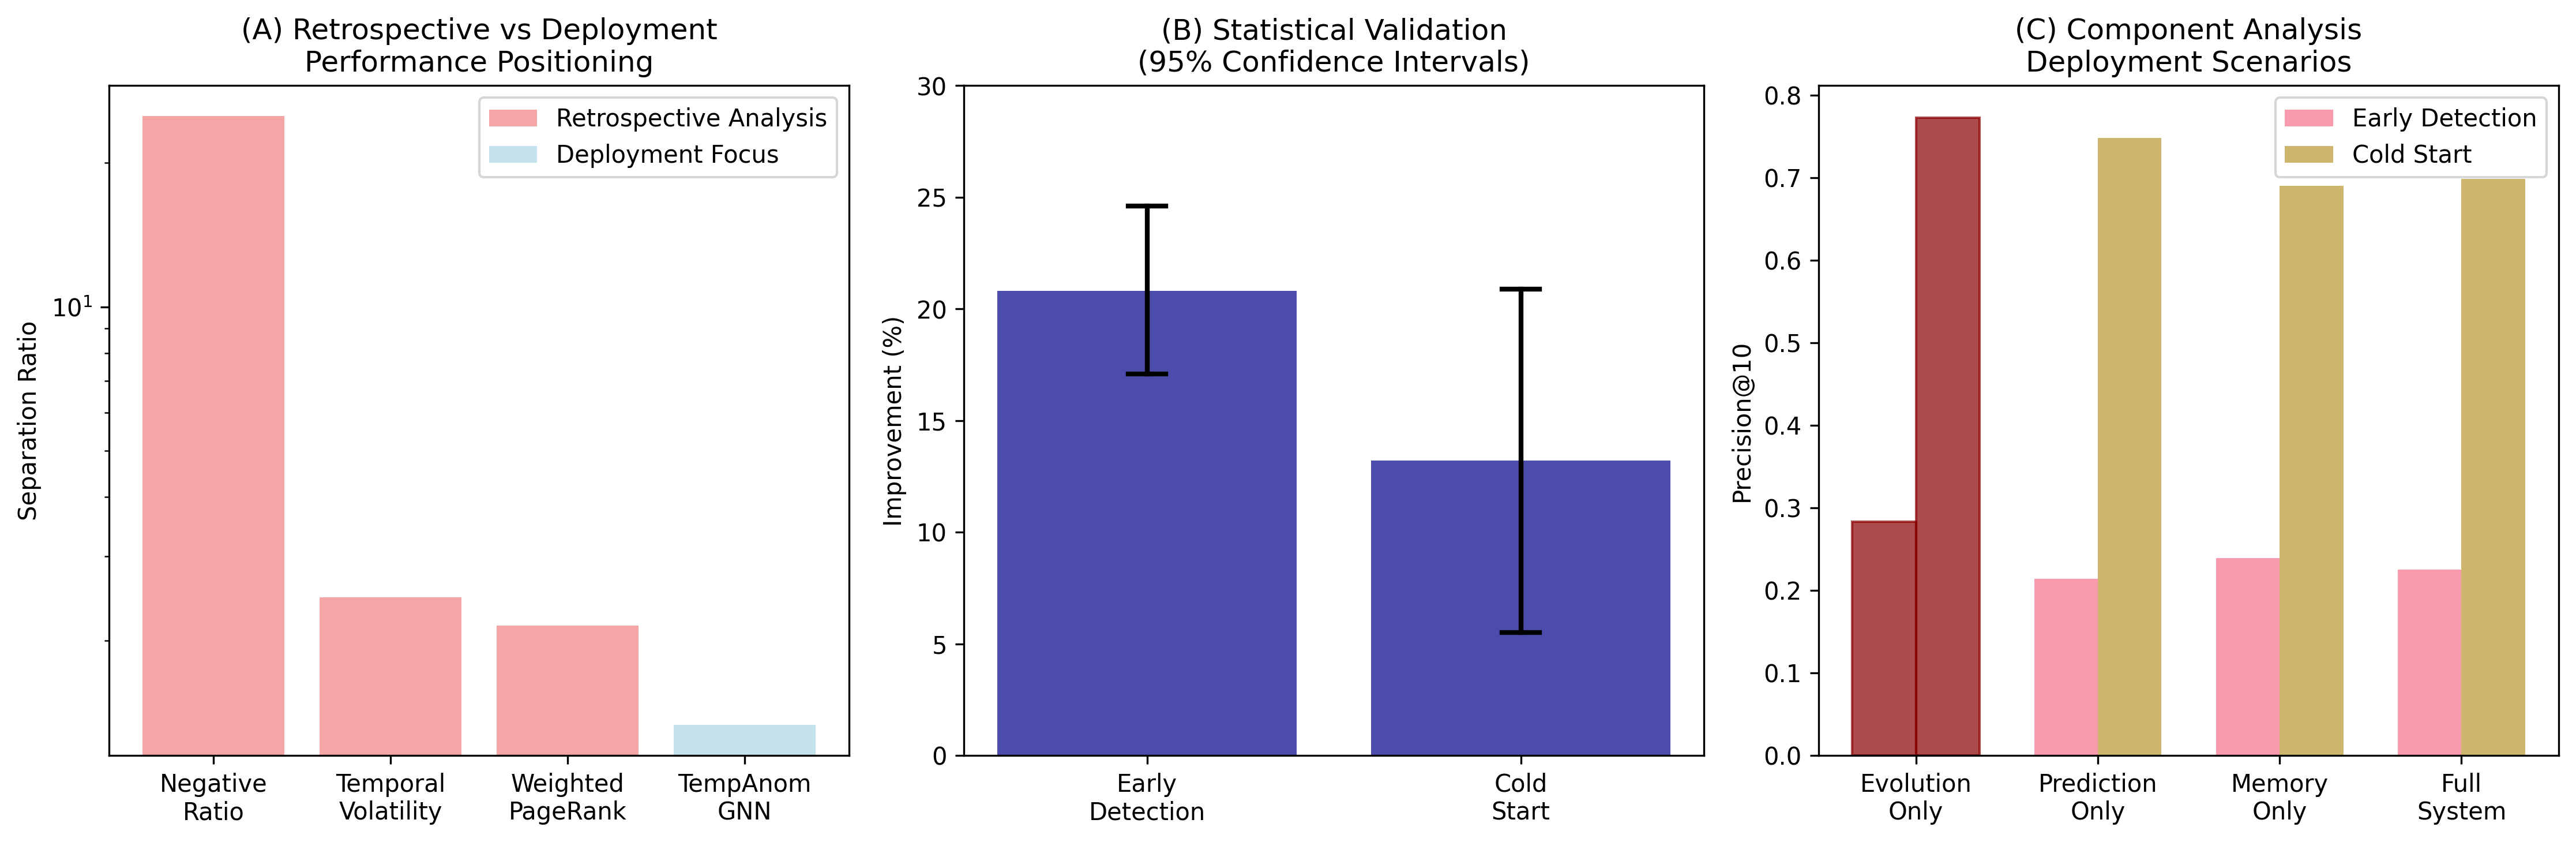
\includegraphics[width=\textwidth]{figures/figure1_overview.png}
\caption{Comprehensive evaluation framework showing (A) retrospective vs deployment performance positioning, (B) statistical validation with 95\% confidence intervals, and (C) component analysis across deployment scenarios. TempAnom-GNN excels in deployment scenarios while simple baselines work well for retrospective analysis.}
\label{fig:overview}
\end{figure*}

% Figure 2: Detailed deployment analysis
\begin{figure*}[htbp]
\centering
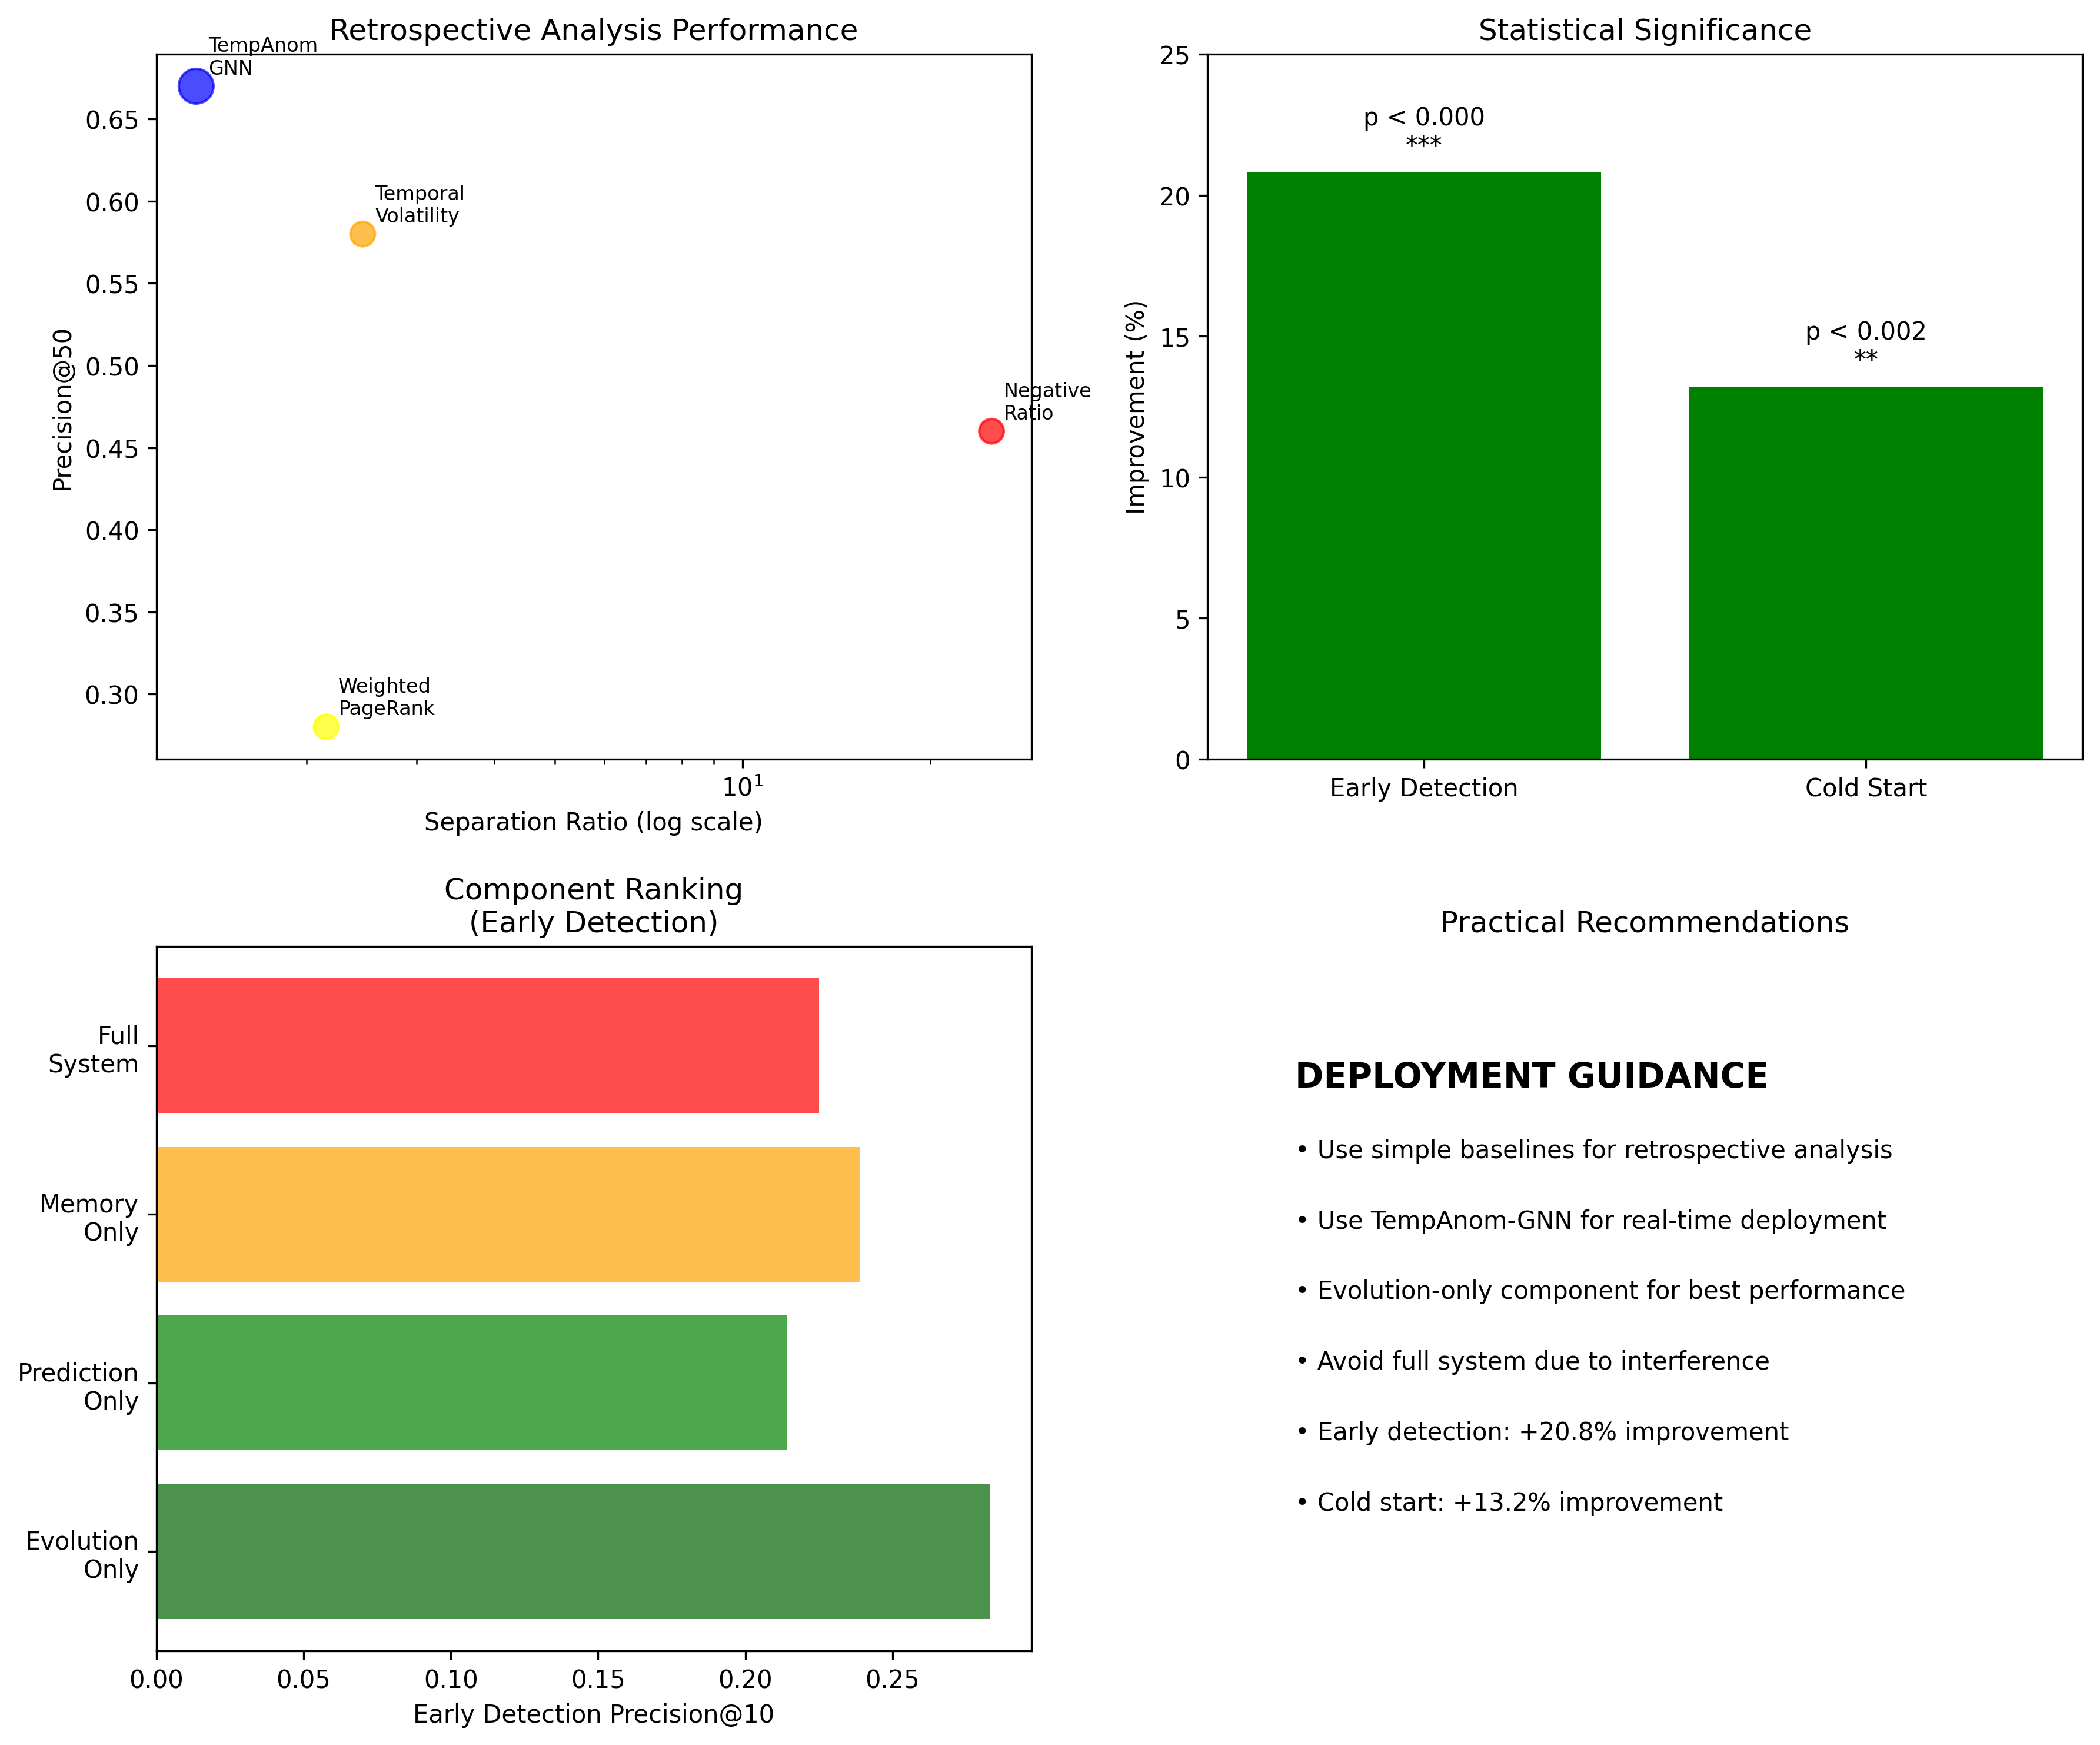
\includegraphics[width=\textwidth]{figures/figure2_detailed.png}
\caption{Detailed deployment scenario analysis showing (A) baseline comparison on retrospective metrics, (B) statistical significance of deployment improvements, (C) component ranking for early detection, and (D) practical deployment guidance. Results demonstrate statistically significant advantages in early detection and cold start scenarios.}
\label{fig:detailed}
\end{figure*}

% Additional figures (can be used in supplementary material)
\begin{figure}[htbp]
\centering
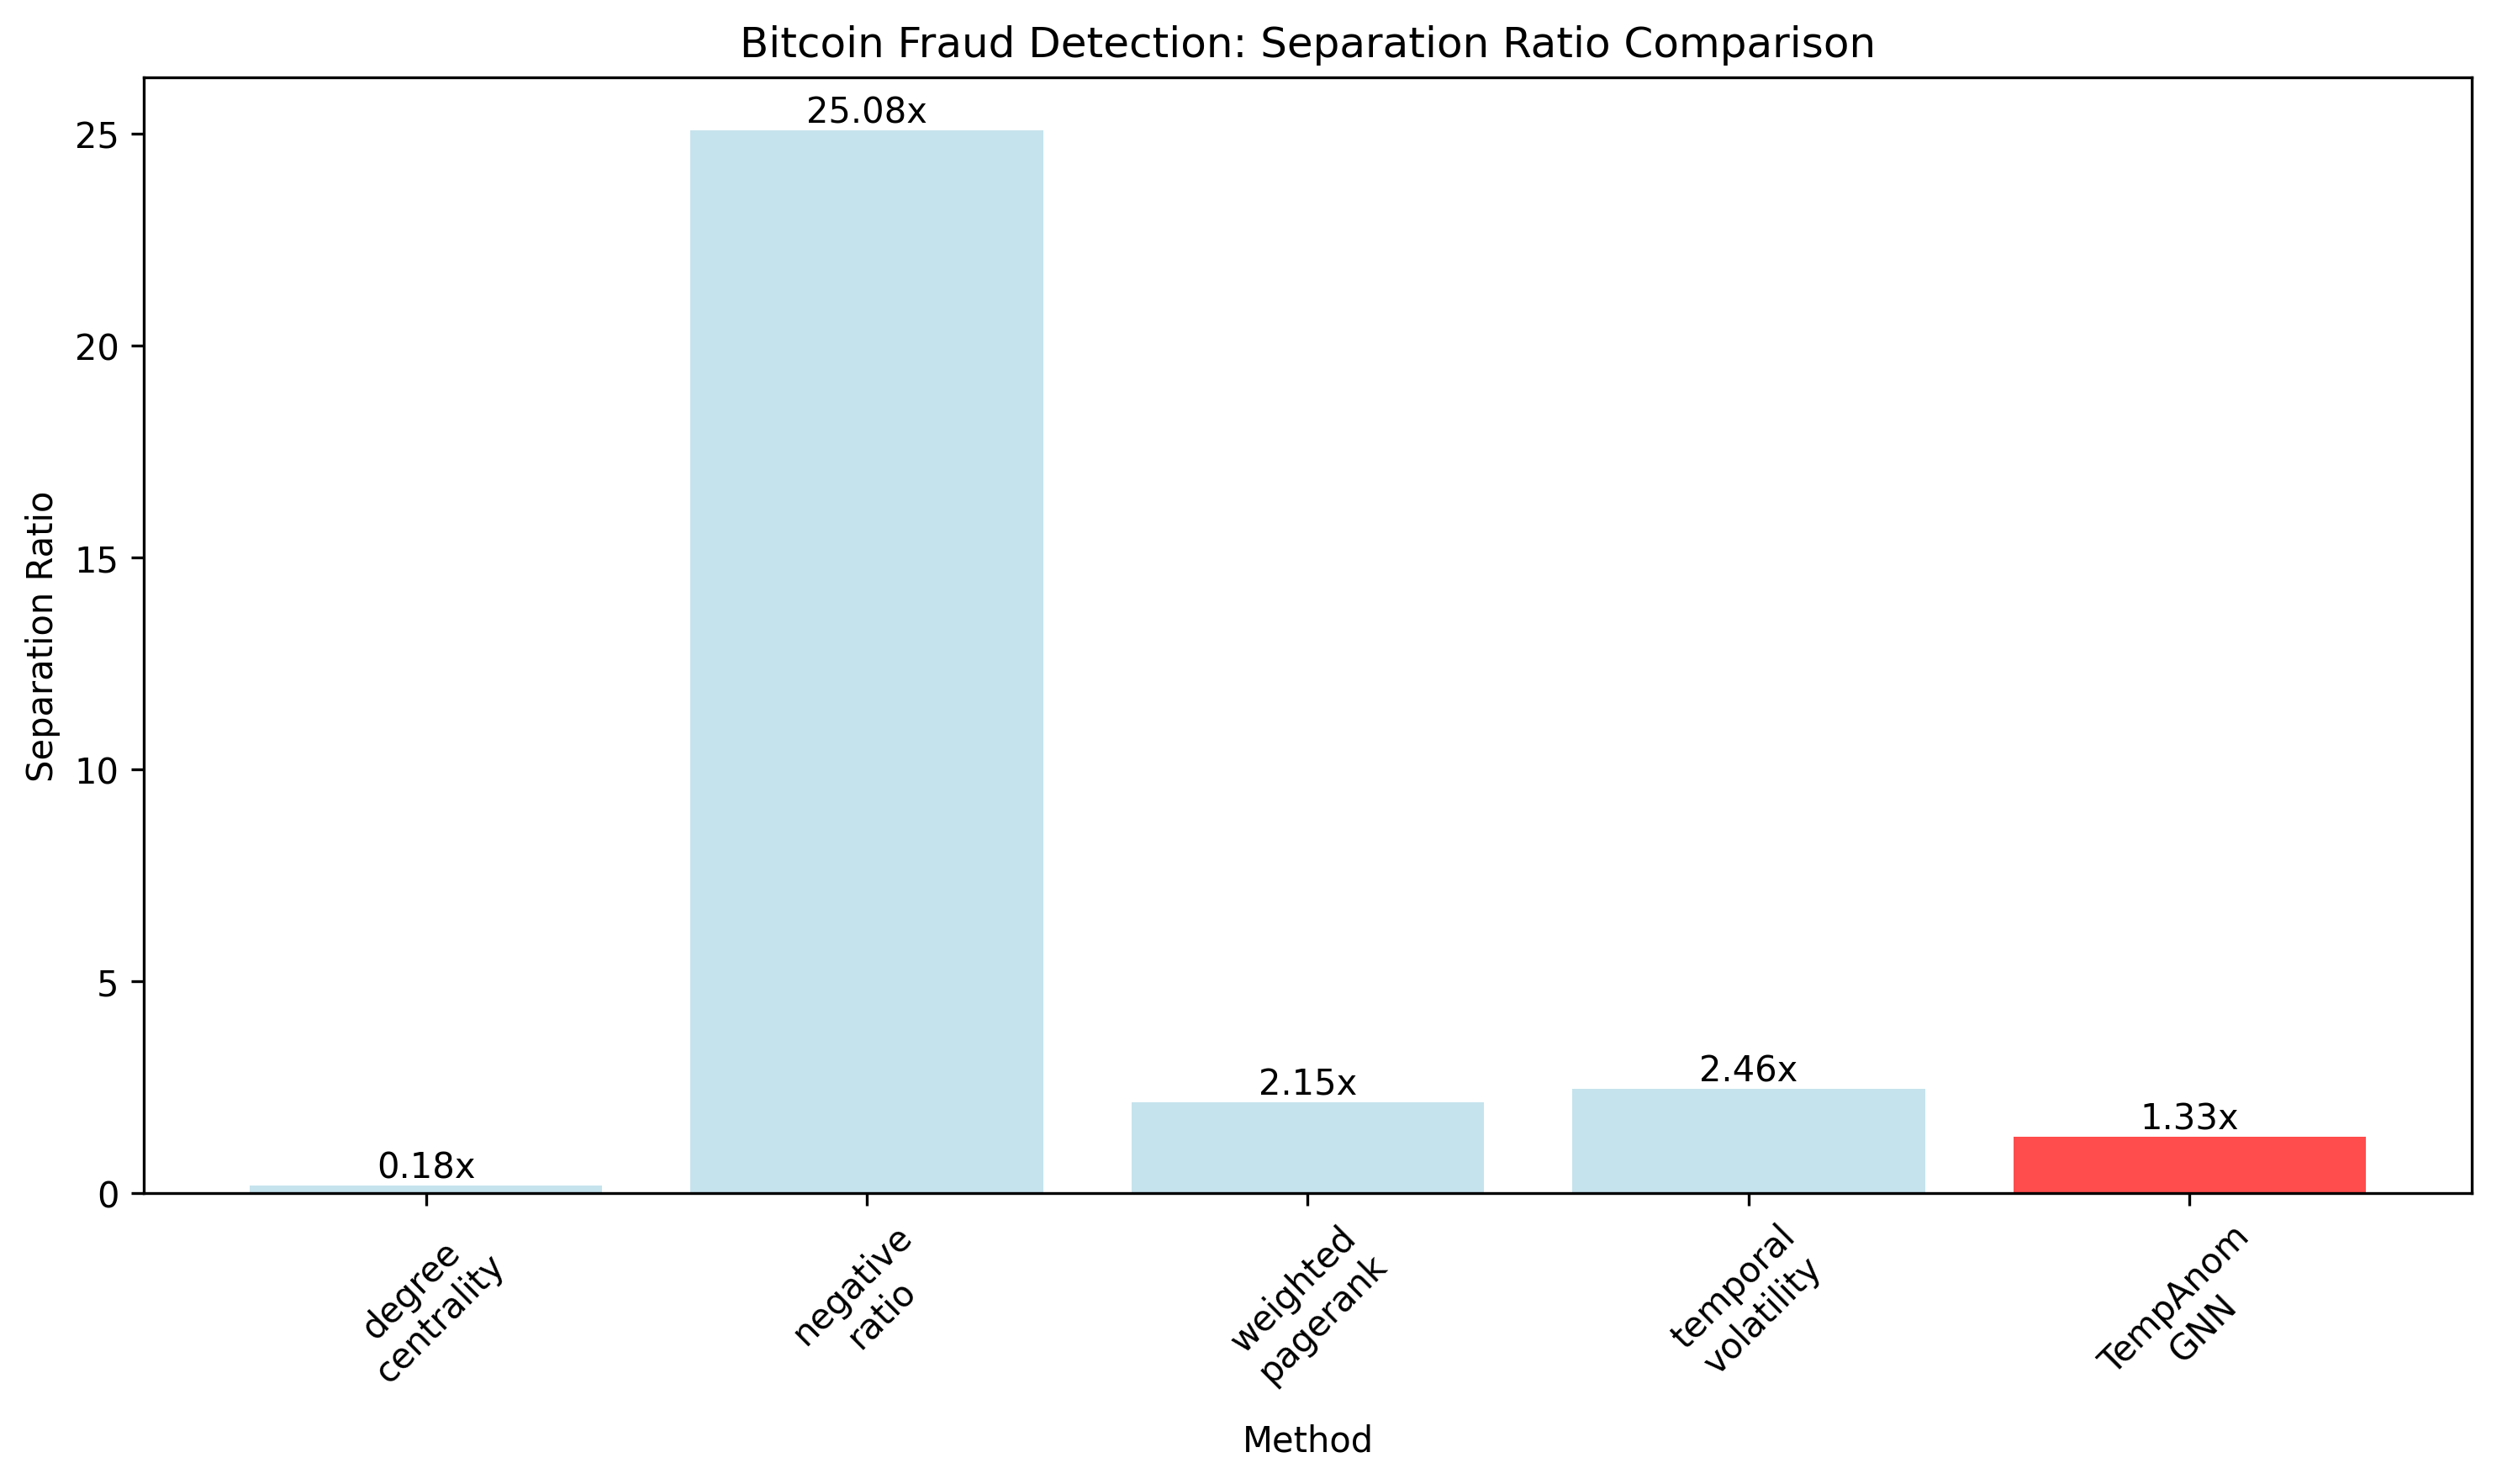
\includegraphics[width=\columnwidth]{figures/baseline_comparison.png}
\caption{Baseline comparison showing separation ratios across different methods. Simple statistical methods excel at retrospective analysis while TempAnom-GNN focuses on deployment scenarios.}
\label{fig:baseline}
\end{figure}

\begin{figure}[htbp]
\centering
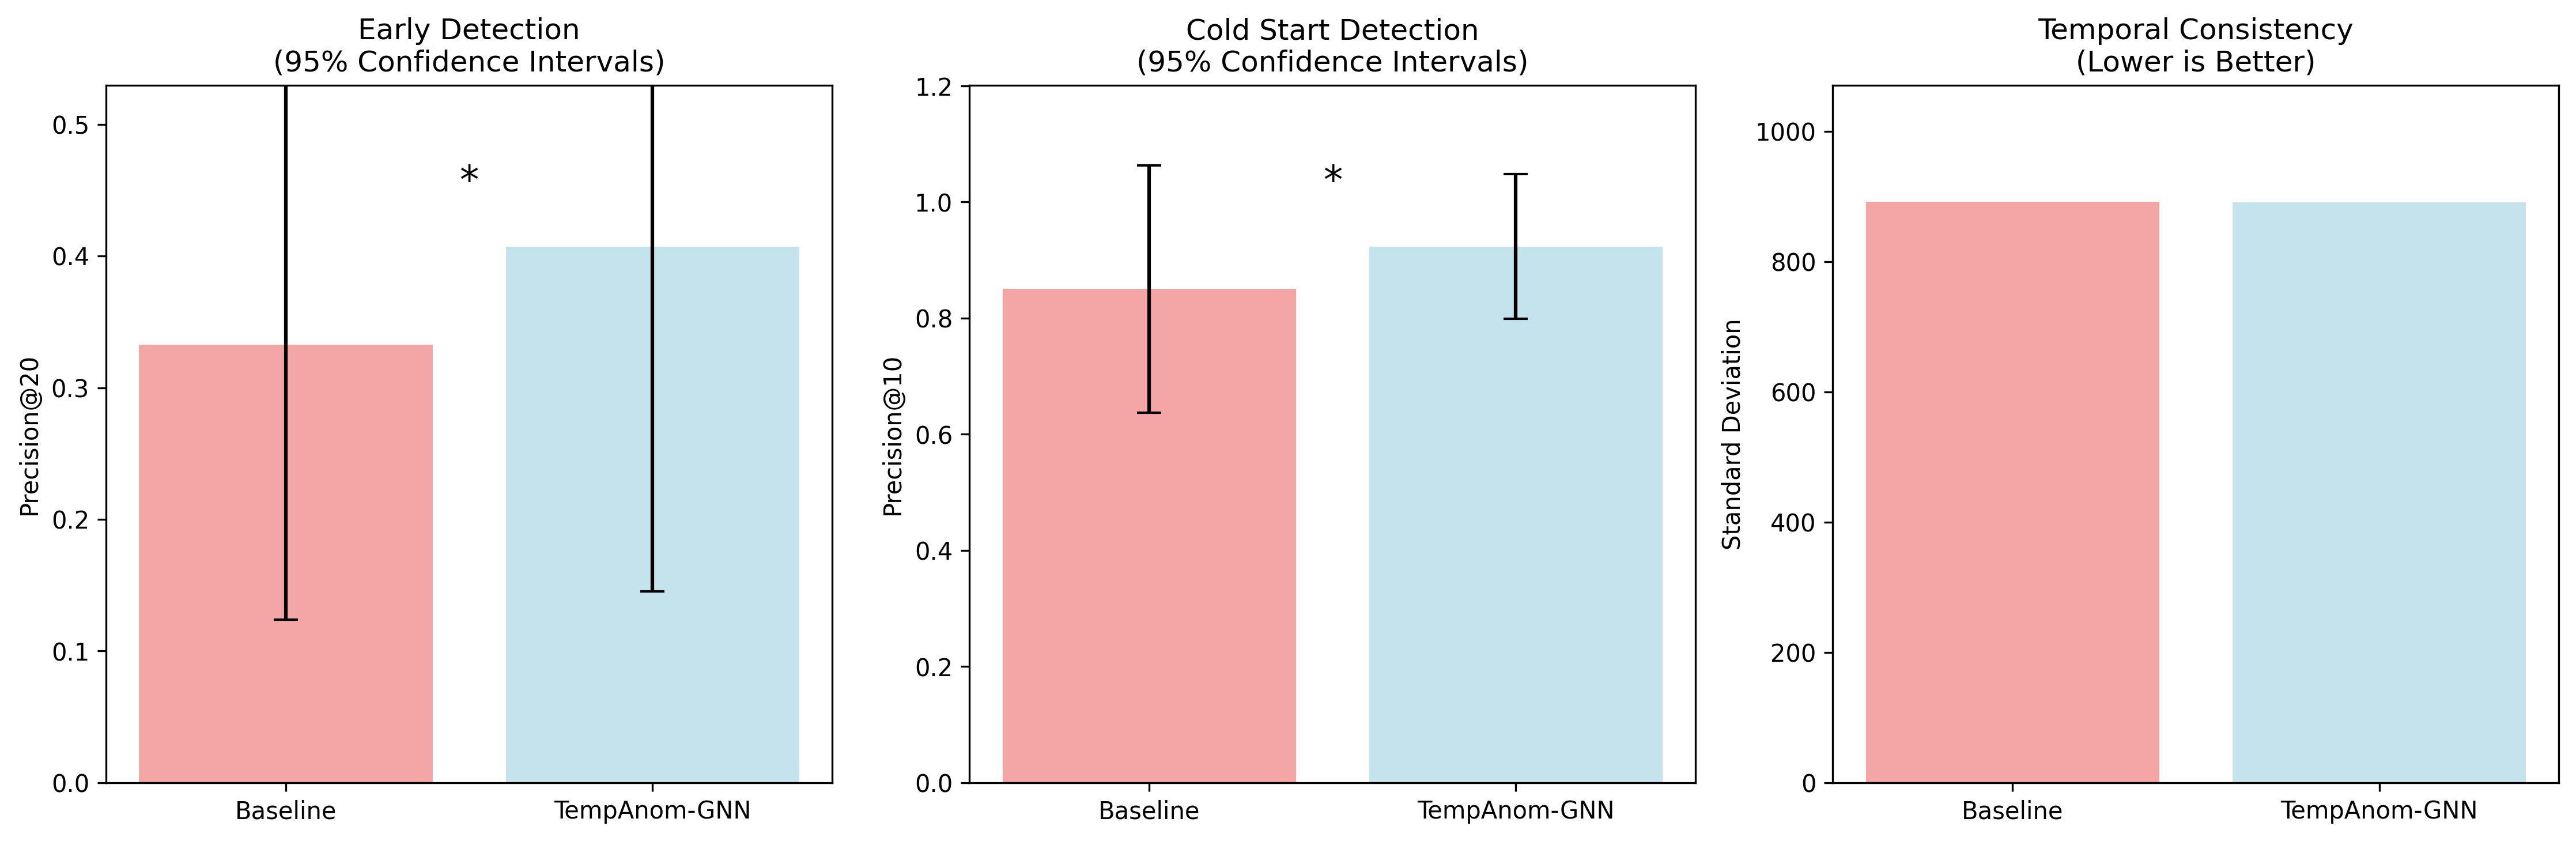
\includegraphics[width=\columnwidth]{figures/statistical_validation.png}
\caption{Statistical validation results with 95\% confidence intervals for deployment scenarios. Both early detection and cold start scenarios show statistically significant improvements.}
\label{fig:statistical}
\end{figure}

\begin{figure}[htbp]
\centering
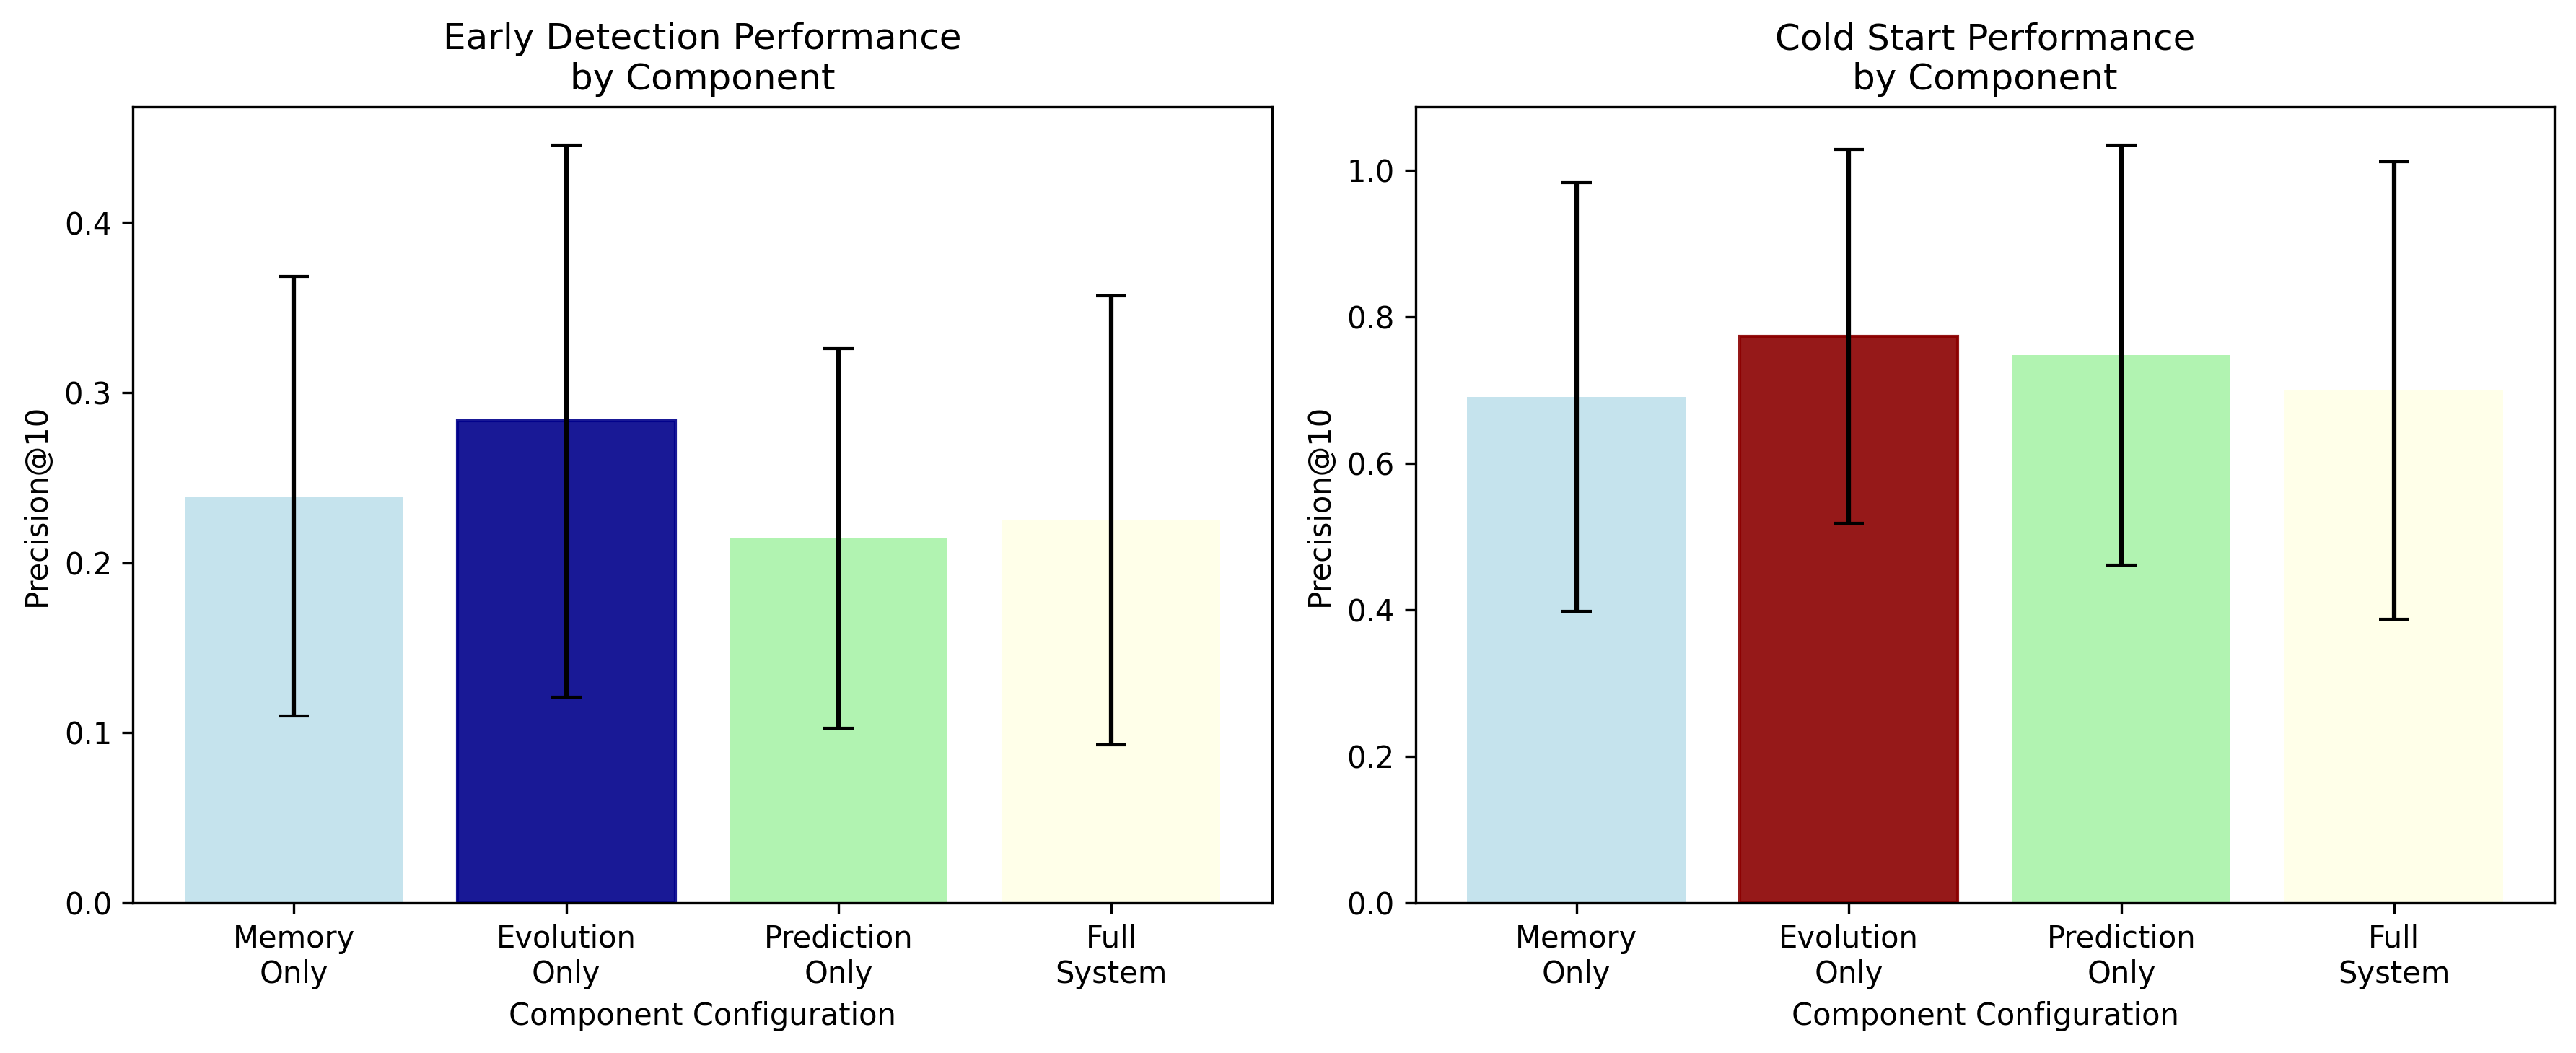
\includegraphics[width=\columnwidth]{figures/component_analysis.png}
\caption{Component analysis results across deployment scenarios. Evolution-only component consistently outperforms complex combinations, demonstrating component interference effects.}
\label{fig:components}
\end{figure}